\documentclass{beamer}
%Для защит онлайн лучше использовать разрешение 16x9
%\documentclass[aspectratio=169]{beamer}

%%% Обязательные пакеты
%% Beamer
\usepackage{beamerthemesplit}
\usetheme{SPbGU}
\beamertemplatenavigationsymbolsempty
\usepackage{appendixnumberbeamer}

%% Локализация
\usepackage{fontspec}
\setmainfont{CMU Serif}
\setsansfont{CMU Sans Serif}
\setmonofont{CMU Typewriter Text}
%\setmonofont{Fira Code}[Contextuals=Alternate,Scale=0.9]
%\setmonofont{Inconsolata}
% \newfontfamily\cyrillicfont{CMU Serif}

\usepackage{polyglossia}
\setdefaultlanguage{russian}
\setotherlanguage{english}
\usepackage[autostyle]{csquotes} % Правильные кавычки в зависимости от языка

%% Графика
\usepackage{wrapfig} % Позволяет вставлять графику, обтекаемую текстом
\usepackage{pdfpages} % Позволяет вставлять многостраничные pdf документы в текст

%% Математика
\usepackage{amsmath, amsfonts, amssymb, amsthm, mathtools} % "Адекватная" работа с математикой в LaTeX

% Математические окружения с русским названием
\newtheorem{rutheorem}{Теорема}
\newtheorem{ruproof}{Доказательство}
\newtheorem{rudefinition}{Определение}
\newtheorem{rulemma}{Лемма}


%%% Дополнительные пакеты. Используются в презентации, но могут быть отключены при необходимости
\usepackage{tikz} % Мощный пакет для создание рисунков, однако может очень сильно замедлять компиляцию
\usetikzlibrary{decorations.pathreplacing,calc,shapes,positioning,tikzmark}

\usepackage{multirow} % Ячейка занимающая несколько строк в таблице

%% Пакеты для оформления алгоритмов на псевдокоде
\usepackage[noend]{algpseudocode}
\usepackage{algorithm}
\usepackage{algorithmicx}

\usepackage{fancyvrb}

%% Пакет для анимированных иллюстраций
\usepackage{animate}


% То, что в квадратных скобках, отображается внизу по центру каждого слайда. 
\title[Реализация RPQ на видеокарте]
{Реализация алгоритма достижимости с регулярными ограничениями на
графическом ускорителе}

% То, что в квадратных скобках, отображается в левом нижнем углу. 
\institute[СПбГУ]{}

% То, что в квадратных скобках, отображается в левом нижнем углу.
\author[Дмитрий Козенко]{Козенко Дмитрий Сергеевич, группа 23.Б08-мм}
 
\begin{document}
{
\setbeamertemplate{footline}{}
% Лого университета или организации, отображается в шапке титульного листа
\begin{frame}
  
\includegraphics[width=1.4cm]{pictures/SPbGU_Logo.png}
\vspace{-35pt}
\hspace{-10pt}
\begin{center}
   \begin{tabular}{c}
        \scriptsize{Санкт-Петербургский государственный университет} \\
        \scriptsize{Кафедра системного программирования}
    \end{tabular}
\titlepage
\end{center}

\btVFill

{\scriptsize
  % У научного руководителя должна быть указана научная степень
   \textbf{Научный руководитель:} : к.ф.-м.н. С.В. Григорьев, доцент кафедры системного программирования
 }
\begin{center}
  \vspace{5pt}
  \scriptsize{Санкт-Петербург\\2025}
  \end{center}
\end{frame}
}

\begin{frame}[fragile]  
  \frametitle{Графовые базы данных и запросы с регулярными ограничениями}
  \begin{itemize}
    \item Графовые базы данных набирают большую популярность в последние дни, например в создании баз знаний\footnote{Zhang Zuopeng Justin. Graph Databases for Knowledge Management \url{https://ieeexplore.ieee.org/document/8123475}}
    \item Запросы с регулярными ограничениями активно используются в графовых базах данных
    \item Нет реализаций алгоритмов для регулярных запросов на GPU
    \item Алгоритм RPQ\footnote{RPQ с линейной алгеброй: \url{https://se.math.spbu.ru/thesis/texts/Beljanin_Georgij_Olegovich_Spring_practice_2nd_year_2024_text.pdf}} основан на операциях линейной алгебры, которые отлично подходят вычислений на GPU
  \end{itemize}
\end{frame}

\begin{frame}  
  \frametitle{Библиотека cuBool\footnote{Репозитория cuBool: \url{https://github.com/SparseLinearAlgebra/cuBool}}}
 
  \begin{itemize}
    \item Достоинства библиотеки
    \begin{itemize}
        \item Она имеет лучшие результаты производительности\footnote{Тесты производительности cuBool: \url{
ht  tps://github.com/SparseLinearAlgebra/cuBool?tab=readme-ov-file\#performance}}
        \item Простота и удобность интеграции и использования
    \end{itemize}
  
    \item Недостатки библиотеки
    \begin{itemize}
        \item Отсутствие поддержки на протяжении долгого времени
        \item Отсутствие одной операции, необходимой для алгоритма
    \end{itemize} 
  \end{itemize} 
\end{frame}

% Обязательный слайд: четкая формулировка цели данной работы и постановка задачи
% Описание выносимых на защиту результатов, процесса или особенностей их достижения и т.д.
\begin{frame}
  \frametitle{Постановка задачи}
  \textbf{Целью} работы является адаптация алгоритма достижимости с регулярными ограничениями для GPGPU вычислений и его перенос на видеокарту

  \textbf{Задачи}:
  \begin{itemize}
      \item Обновить библиотеку cuBool для поддержки последней версии CUDA
      \item Реализовать в cuBool недостающие для алгоритма операции с булевыми матрицами
      \item Реализовать алгоритм, используя обновленную библиотеку
      \item Провести эксперименты: найти узкие места в алгоритме и уменьшить среднее время исполнения, сравнить время работы реализации алгоритма на GPU с его реализацией на CPU и проанализировать результаты
  \end{itemize}
\end{frame}
 
%Идеально, если есть по одному слайду на каждую поставленную задачу            

\begin{frame}  
  \frametitle{Обновление cuBool}

  \begin{itemize}
     \item Библиотека cuBool была обновлена с версии CUDA 10.1 от 28 июля 2019 года до версии 12.6 от 14 августа 2024 года
     \item Удалена локальная версия Cub, который в последней версии CUDA устанавливается вместе с ней в систему
     \item Удалена опция компиляции \textit{CUDA\_SEPARABLE\_COMPILATION}
\footnote{Документация cmake: \url{https://cmake.org/cmake/help/latest/prop_tgt/CUDA_SEPARABLE_COMPILATION.html}}
из CMake, из-за которой многие тесты вели себя недетерминировано и падали
  \end{itemize} 
\end{frame}

\begin{frame}  
    \frametitle{Реализация недостающей опции}

    \begin{itemize}
        \item B cuBool не хватает операции умножения на инвертированную матрицу, необходимую для применения маски посещенных состояний.
        \item Все матрицы в cuBool в силу разреженности хранятся как множество индексов ненулевых элементов
        \item Пусть $C = A * \overline{B}$. Посмотрим, когда конкретный элемент $C$ ненулевой
$$
C_{ij} = 1
\Longleftrightarrow
\begin{cases}
    A_{ij} = 1 \\
    \overline{B_{ij}} = 1
\end{cases}
\Longleftrightarrow
\begin{cases}
    A_{ij} = 1 \\
    B_{ij} = 0
\end{cases}
\Longleftrightarrow
\begin{cases}
    A_{ij} = 1 \\
    B_{ij} \ne 1
\end{cases}
$$
    \item Множество ненулевых индексов $C$ равно разности множеств ненулевых элементов матриц $A$ и $B$
    \end{itemize}
    
\end{frame}

\begin{frame}  
    \frametitle{Реализация алгоритма}

    \begin{itemize}
        \item Обновлена библиотека cuBool, результат работы можно увидеть в форке\footnote{Форк репозитории cuBool: \url{https://github.com/mitya-y/cuBool}} на GitHub на ветке \textit{update-cuda-12.6}
        
        \item Реализован алгоритм, код находится в репозитории\footnote{Репозитория с алгоритмом: \url{https://github.com/mitya-y/rpq}} GitHub
        
        \item Настроен CI в репозитории:
            \begin{itemize}
                \item Запуск тестов на версии функций cuBool, делающих вычисления на CPU
                \item Запуск проверки стиля кода анализатором \textit{clang-format}
            \end{itemize}
    \end{itemize}     
\end{frame}


\begin{frame}[t]
  \frametitle{Условия эксперимента}
  \begin{itemize}
    \item В качестве данных была выбрана база знаний \textsc{Wikidata}\footnote{База знаний \textsc{WikiData}: \href{https://www.wikidata.org/wiki/Wikidata:Database_download}{https://www.wikidata.org/wiki/Wikidata:Database\_download} (Дата доступа 11.12.24)} --- граф размером 270 миллионов вершин, 15 миллиардов
рёбер, а также 600 регулярных запросов к нему
    
    \item Для замера времени работы реализации на CPU оригинальный тест производительности из репозитория GitHub\footnote{Код для теста производительности алгоритма: \url{https://github.com/georgiy-belyanin/RPQ-bench}}
    
    \item Для реализации на GPU был написан схожий тест производительности\footnote{Код теста: \url{
    https://github.com/mitya-y/rpq/blob/master/benchmark.cpp}}
    
    \item Тесты проводились на машине с Intel i5-10400f и Nvidia RTX 3050 (8 Gb VRAM), 16 Gb RAM
  \end{itemize}  
\end{frame}


\begin{frame}[t]
  \frametitle{Результаты сравнения с реализацией на CPU}
  
\begin{figure}[H]
    \centering
    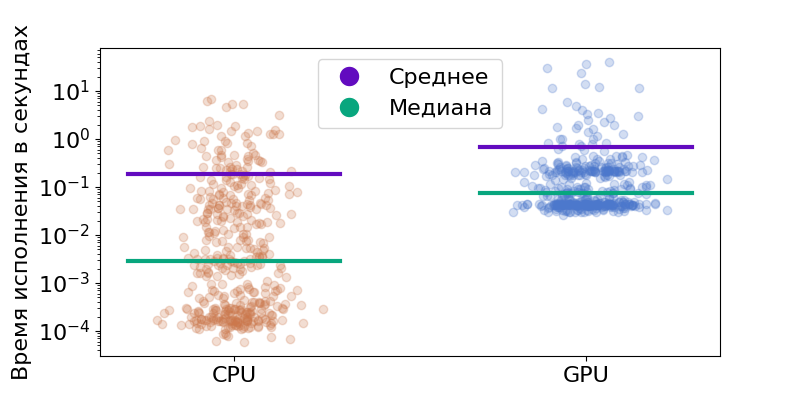
\includegraphics[scale = 0.57]{pictures/Cloud.png}
    \caption{Облако распределения времени исполнения запросов}
    \label{GraphicFull}  
\end{figure}
    
\end{frame}


\begin{frame}[t]
  \frametitle{Результаты сравнения с реализацией на CPU}
  
\begin{figure}[H]
    \centering
    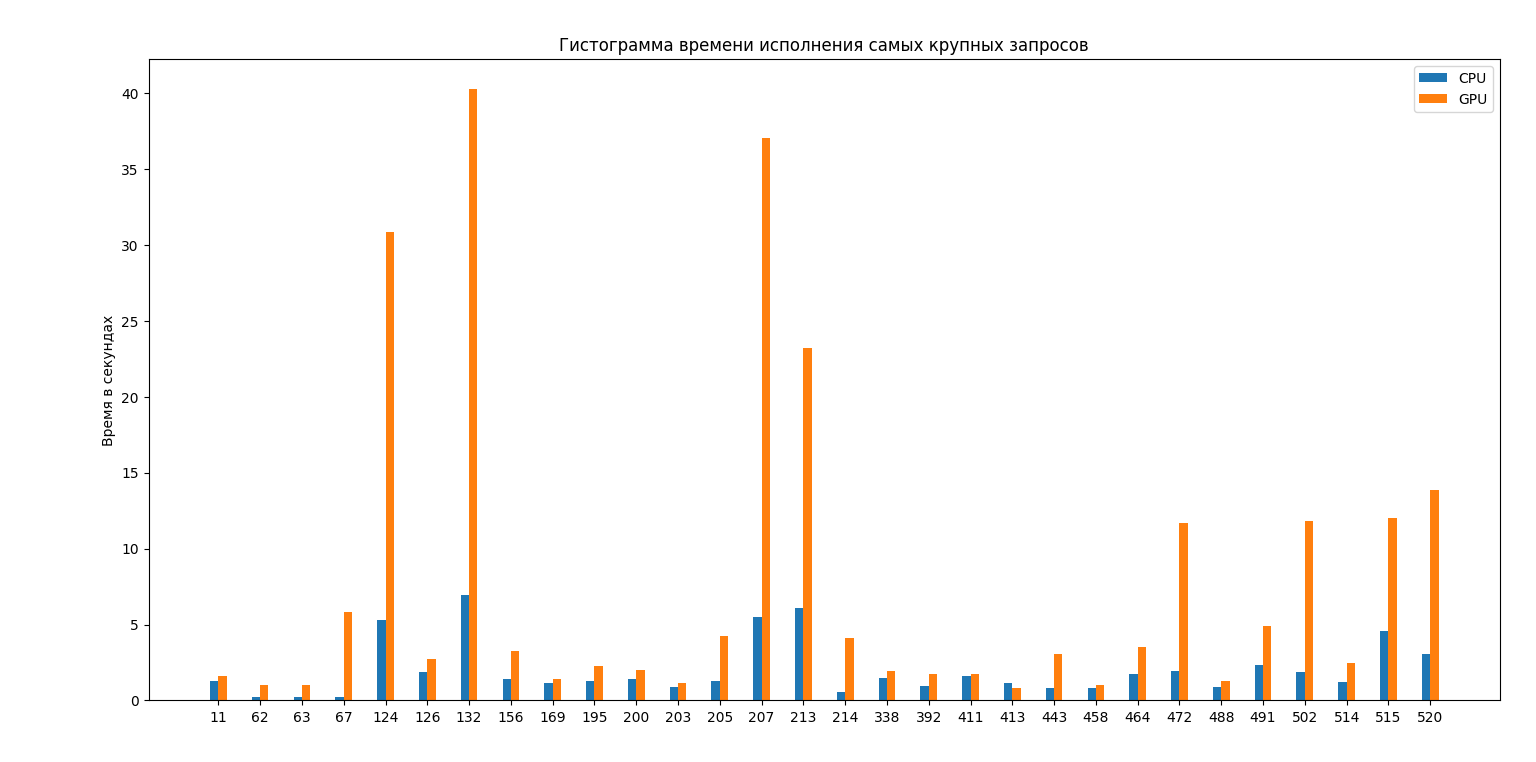
\includegraphics[scale=0.3]{pictures/HistBig.png}
    \caption{Гистограмма времени исполнения на самых крупных запросах (занявших более 1 секунды)}
\end{figure}
   
\end{frame}

\begin{frame}[t]
  \frametitle{5 лучших и 5 худших запросов в сравнении с CPU}

\begin{table}[]
\centering
\scalebox{0.7}{
    \begin{tabular}{|c|c|}
    \hline
         Среднее замедление & 3.59 \\ 
    \hline
         Медиана всех ускорений & 0.0379 \\
    \hline
         Среднее аримф. по всем ускорениями & 0.232 \\
    \hline
    \end{tabular}
}
\end{table}
 
\begin{table}[]
\centering
\scalebox{0.7}{
    \begin{tabular}{|c|c|c|c|}
    \hline
         Номер запроса & Время GPU & Время CPU & Ускорение \\
    \hline
        353 & 0.182 & 0.263 & 1.444 \\
        421 & 0.294 & 0.441 & 1.501 \\
        416 & 0.431 & 0.704 & 1.633 \\
        346 & 0.277 & 0.46  & 1.658 \\
        311 & 0.179 & 0.3   & 1.682 \\
    \hline
    \end{tabular}
}
    \caption{5 лучших запросов}
\end{table}

\begin{table}[]
\centering
\scalebox{0.7}{
    \begin{tabular}{|c|c|c|c|}
    \hline
         Номер запроса & Время GPU & Время CPU & Ускорение \\
    \hline
        429 & 0.170 & 0.000081 & 0.000476 \\
        511 & 0.200 & 0.000111 & 0.000553 \\
        484 & 0.202 & 0.000127 & 0.000627 \\
        433 & 0.175 & 0.000118 & 0.000671 \\
        442 & 0.174 & 0.000119 & 0.000683 \\
    \hline
    \end{tabular}
}
    \caption{5 худших запросов}
\end{table}

\end{frame}
 
\begin{frame}
  \frametitle{Результаты}

\begin{itemize}
    \item Библиотека cuBool была обновлена до последней версии CUDA
12.6
    \item В cuBool реализована операция поэлементного умножения на ин-
вертированную матрицу
    \item При помощи обновленной версии cuBool алгоритм достижимости
с регулярными ограничениями был реализован для запуска на
GPU
    \item Был проведен эксперимент, который показал, что текущая реали-
зация на GPU проигрывает в производительности реализации на
CPU: абсолютное среднее замедление равно 3.59
\end{itemize}


\end{frame}

\end{document}
